\chapter{Parameters of the Reaction Wheel}\label{app:wheelParameters} 
\textbf{Group 630}

\subsubsection{Purpose}
Provide a method to measure and estimate the wheel's mass, distance to the frame's pivoting point, inertia and friction to include these parameters in the model instead of previous groups'.

\subsubsection{Setup and Principle}

To measure the mass of the wheel, a scale can be used if the wheel is dismantled from the setup. To get the distance from the center of the wheel to the pivoting point of the frame, a precise ruler can be used.
The setup needed to estimate the wheel's inertia and friction can be seen on \figref{fig:wheelParameterTestSetup}.
\begin{figure}[H]
  \centering
  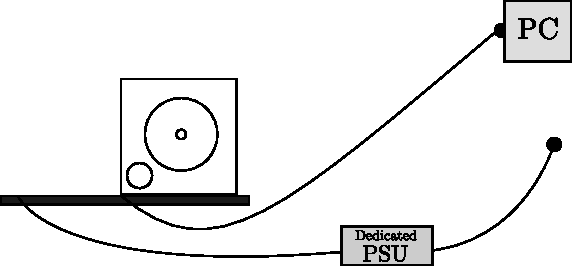
\includegraphics[scale=1]{figures/wheelParameterTestSetup}
  \caption{Setup diagram}
  \label{fig:wheelParameterTestSetup}
\end{figure}

By applying a current step to the motor, and measuring the output velocity, as shown on \figref{Parameters}, it is possible to use Senstools in a similar way to how it is used in \secref{sec:parameterEstimationUsingOptimization} with a Simulink model of the wheel and the attached motor. The inertia and friction parameters of the simulation model will be fitted to match the reality on this test.

\begin{figure}[H]
    \begin{tikzpicture}[ auto,
						thick,                         %<--setting line style
						node distance=2cm,             %<--setting default node distance
						scale=1.0,                     %<--|these two scale the whole thing
						every node/.style={scale=1.0}, %<  |(always change both)
						>=triangle 45 ]                %<--sets the arrowtype
  ]
  
  %-- Blocks creation --%
  \draw
	node[shape=coordinate][](ref) at (0,0){}			% start of reference
 
	node(K) at (2,0) [block] {\si{K_t}}
	
	node(sum) at (4,0) [sum] {$\sum$}
	
	node(J) at (6,0) [block] {\si{\frac{1}{J_w}}}
	
	node(int) at (8,0) [block] {\si{\frac{1}{s}}}
	
	node[shape=coordinate][](velFeed) at (9,0){theta\_w}
	
	node[shape=coordinate][](out) at (10,0){theta\_w}
	
	% - feedback nodes
	node(B) at (7,-1.5) [block] {\si{B_w}}
	
  ;
  
  \draw[->](ref) -- node {\si{i}} (K);
  
  \draw[->](K) -- node {\si{\tau}} (sum);
   
  \draw[->](sum) -- node {} (J);
  
  \draw[->](J) -- node {\si{\ddot{\theta}_w}} (int);
  
  \draw[->](int) -- node {\si{\dot{\theta}_w}} (out);
  
  % - drawing feedback lines
  
  \draw[-](velFeed) |- node {} (B);
  
  \draw[-](B) -| node {} (sum);
  
  % - adding + and - at the sum nodes
    \draw 
  node at (sum) [right = -6.6mm, below = .6mm] {$+$}
  node at (sum) [right = -3mm, below = 3.9mm]  {$-$} 
  ;
 
  
  \end{tikzpicture}
  \centering
  \caption{Block diagram of the wheel used for the simulation}
  \label{Parameters}
\end{figure}


\subsubsection{List of Equipment}
\begin{table}[H]
  \begin{tabular}{|l|l|}
    \hline%------------------------------------------------------------------------------------------------------------
    \textbf{Instrument}                                    &  \textbf{Type}            \\
    \hline%------------------------------------------------------------------------------------------------------------
    Dedicated Power Supply of Cubli \small{(24 V - 3 A)}                     &  XP Power, AEB70US24      \\
    \hline%------------------------------------------------------------------------------------------------------------
    Probe                                                                    &  1:1                      \\
    \hline%------------------------------------------------------------------------------------------------------------
    Computer                                        &                           \\
    \hline%------------------------------------------------------------------------------------------------------------
  \end{tabular}
\end{table}

\subsubsection{Procedure}
\begin{enumerate}
  \item Plug the dedicated Power Supply Unit to the Cubli setup, then to the computer.
  \item Prepare the code so that a current step is applied to the motor after a certain amount of time and the velocity of the wheel and the actual current are logged into a file. Upload this program to the BeagleBone Black.
  \item Fix the frame tightly so that it doesn't move during the test.
  \item Launch the test program and wait a few seconds after the activation of the motor so that the wheel's velocity seems to saturate.
  \item Stop the program. Gather the CSV log file generated by the program, from the BeagleBone Black.
  \item It is possible to repeat the last two steps multiple times to have a set of tests to compare.
  \item Use the data to fit the model in Simulink with Senstools.
\end{enumerate}